\chapter{State of the art}
\label{chap:sota}

\section{Object detection}

Object detection is one of the most fundamental and challenging problems in computer vision \cite{zou2019object}. This task can be define as follows: given an image, determine whether or not there are instances of a predefined set of objects, usually referred as classes, and, if present, return the location of each instance \cite{liu2020deep}. The spatial location of an object in an image can be represented using bounding boxes.

Object detection has initially been addressed using handcrafted features and shallow trainable architectures.
With the rapid development in deep learning, more powerful techniques are used to address the problems existing in traditional architectures \cite{zhao2019object}. 

As described in \cite{zhao2019object}, the frameworks of object detection methods can mainly be categorized into two types:
\begin{enumerate}
    \item Generating region proposals at first and then classifying each proposal into different object categories.
    \item Adopting a unified framework to achieve final results (categories and locations) directly.
\end{enumerate} 

\subsection{YOLO}
YOLO \cite{redmon2016you} is a model for object detection composed of a single neural network which treats object detection as a regression problem: given an image as input it produces bounding box coordinates and associated class probabilities. Since the predictions are performed directly on the input image without requiring complex pipelines, YOLO (you only look once) is very efficient and can lead to real-time object detection.

\begin{figure}
    \begin{center}
        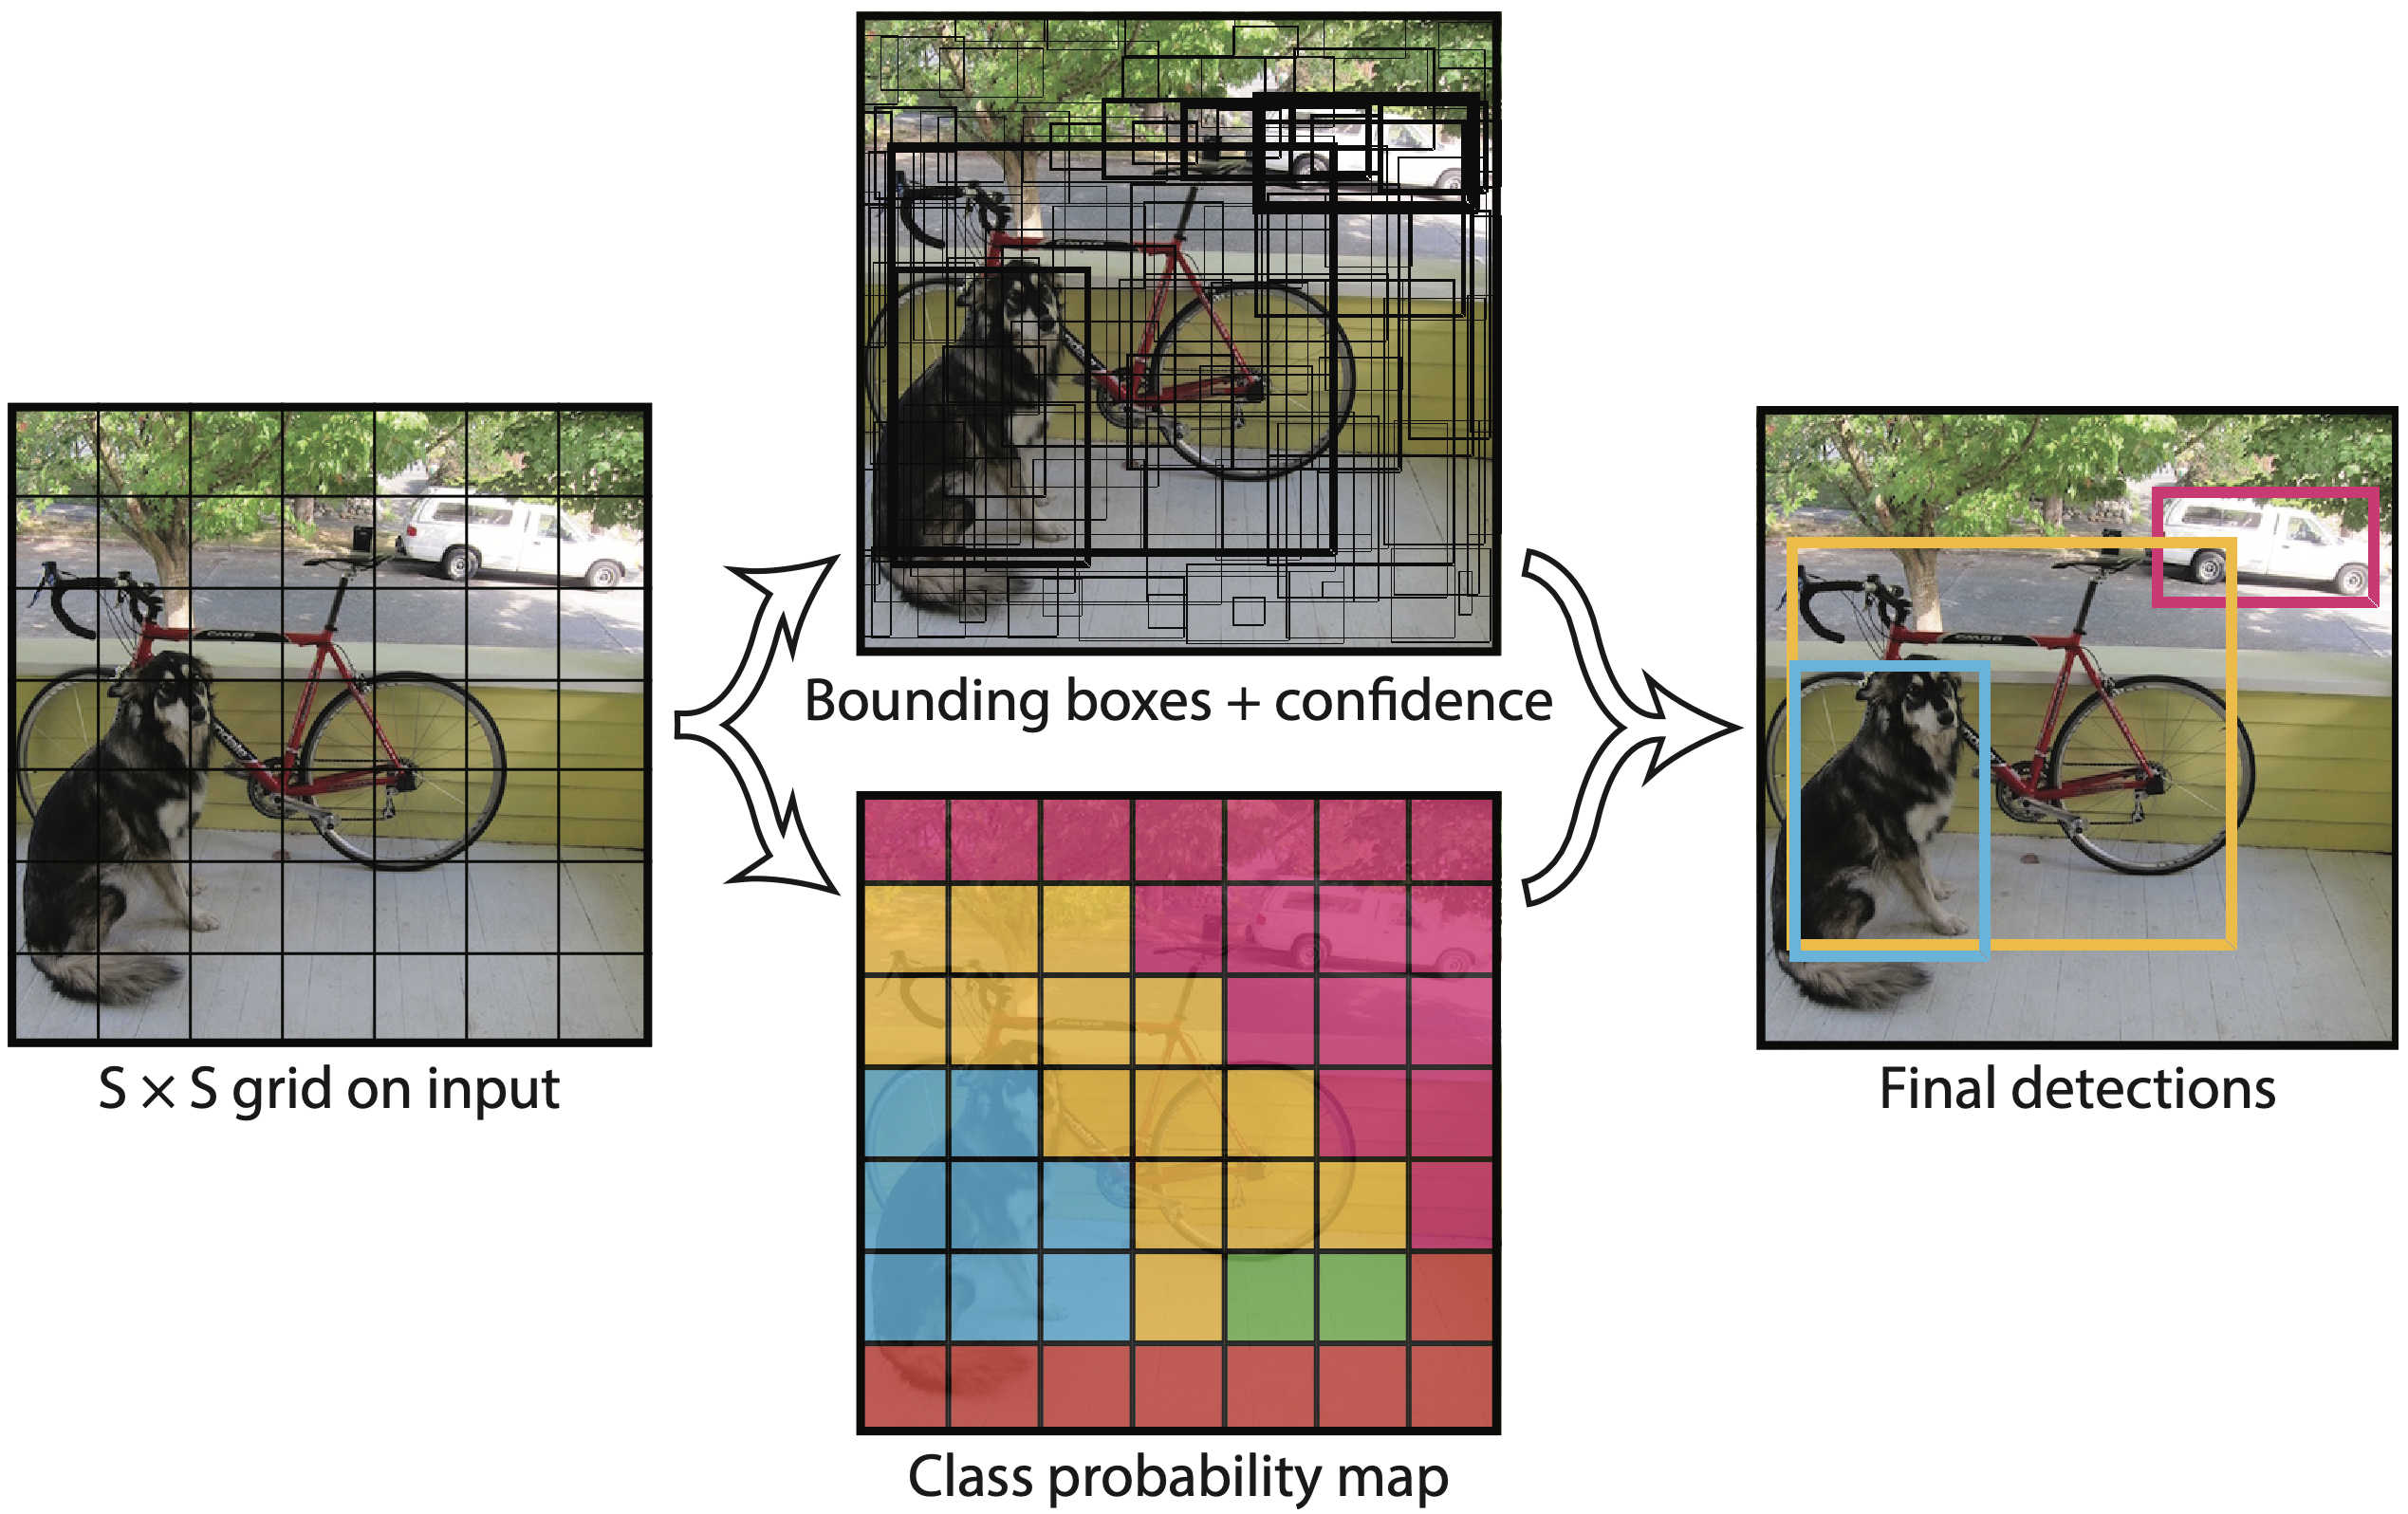
\includegraphics[width=\columnwidth]{images/yolo-model.png}
    \end{center}
    \caption{Pipeline of YOLO presented in \cite{redmon2016you}.}
    \label{fig:yolo-model}
\end{figure}

In YOLO, the input image is divided into a $S \times S$ grid and the cell in which the center of the object falls is responsible for the detection of that object.
A grid cell can predict more than one bounding box, where each prediction consists of an array composed by 5 elements: center of the bounding identified by the coordinates $x$ and $y$, dimensions of the box $w$ and $h$, and the confidence score of that bounding box representing and object. At the same time, regardless of the number of boxes in each cell, C conditional probabilities $\Pr(Class_i | Object)$ are computed in each grid cell. The final prediction will be encoded as an $S \times S \times (B * 5 + C)$ tensor. The model pipeline is shown in \autoref{fig:yolo-model}

The model is trained via the optimization of the following loss function:

\begin{equation}\label{eq:yolo-loss}
    \begin{split}
        \mathcal{L} \quad =  \quad  &
            \lambda_{coord} \sum_{i=0}^{S^2} \sum_{j=0}^{B} \mathbb{1}_{ij}^{obj}
            [(x_i - \hat x_i)^2 + (y_i - \hat y_i)^2]\\
            \quad + \quad & \lambda_{coord} \sum_{i=0}^{S^2} \sum_{j=0}^{B} \mathbb{1}_{ij}^{obj}
                [(\sqrt{w_i} - \sqrt{\hat w_i})^2 + (\sqrt{h_i} - \sqrt{\hat h_i})^2]\\
            \quad + \quad & \sum_{i=0}^{S^2} \sum_{j=0}^{B} \mathbb{1}_{ij}^{obj}
                (C_i - \hat C_i)^2 \; + \; \lambda_{noobj} \sum_{i=0}^{S^2} \sum_{j=0}^{B} \mathbb{1}_{ij}^{noobj}(C_i - \hat C_i)^2\\
            \quad + \quad & \sum_{i=0}^{S^2} \mathbb{1}_{i}^{obj} \sum_{c \in classes}
                (p_i(c) - \hat p_i (c))^2\\
    \end{split}
\end{equation}
where,
\begin{align*}
    \mathbb{1}_{ij}&=\left\{
        \begin{array}{@{}ll@{}}
            1, & \text{if the } j \text{-th bbox in cell } i \text{ is responsible fot that prediction}\\
            0, & \text{otherwise}
        \end{array}\right.\\
    \mathbb{1}_{i}&=\left\{
        \begin{array}{@{}ll@{}}
            1, & \text{if there is an object in cell}\ i \\
            0, & \text{otherwise}
        \end{array}\right.
\end{align*}


The loss function in \autoref{eq:yolo-loss} considers both detection and classification. A bounding box can be defined by its center in addition to the height and width. The first row of the loss function is responsible for minimizing the difference between the predicted center and the ground truth, and the second row minimize the difference between width and height.
The third row penalizes the neural network if it predicts an object whereas it is not present and vice versa. The last row of the loss function is the mean squared error between the real class and the predicted one, hence it is responsible to match the real class.


Over the years, several versions of YOLO have came up, starting from the first up to fifth versions \cite{redmon2016you, redmon2017yolo9000, redmon2018yolov3, bochkovskiy2020yolov4, glenn_jocher_2021_5563715}. YOLOv5 represents the state of the art for object detection, and compared with the most recent detectors architectures it is among the best performing models \cite{zaidi2022survey}.

\section{Logo recognition}
\label{sec:sota-logoyolo}

A general pipeline for logo detection and recognition consists in logo region proposal followed by a classifier specifically trained for logo classification, as proposed by Bianco et al. in \cite{bianco2017deep} or by Fehérvári et al. in \cite{fehervari2019scalable}.

Another approach presented by Wang et al. \cite{wang2022logodet} involve a model based on YOLOv3 \cite{redmon2018yolov3} used to produce both bounding boxes and classification for each detected logo. The proposed model is called Logo-YOLO, which is essentially the same version of YOLOv3 with some changes to the loss function and the re-computation of the anchors sizes. The modified loss function utilizes the Focal Loss \cite{lin2017focal} to solve the problem of logos usually begin small object relative to the background, and the  CIoU loss \cite{zheng2020distance} to obtain more accurate regression results.

The issue with this approaches is the closed-world assumption which does not apply in the case of logo recognition, as discussed in \autoref{sec:logodet-intro}. This is the motivation behind works such as \cite{fehervari2019scalable}. The authors of the paper propose a method based on Distance Metric learning (DML) using deep learning techniques called SoftTriple Loss and presented in \cite{qian2019softtriple}. This work aims to achieve logo recognition via metric learning, where a model learns the similarity among arbitrary groups of data, thus being able to deal with a large number of previously unseen classes.

Another work based on DML has been presented by Li et al. \cite{li2022seetek} and can be considered as an extension to \cite{fehervari2019scalable}. In this work the author enrich the latent space learned by DML with text features contained in the logos. The authors point out how many logos have remarkable amount of text or (stylized) letters, for this reason they consider both visual and text features for logo classification.

\section{Class incremental learning}
Traditional supervised learning systems are trained in closed-world for a fixed
number of classes, that requires all the training data to be available before training.
The problem of class incremental learning (CIL) aims to design algorithms that can learn new concepts in a sequential way and eventually perform well on all observed classes \cite{yan2021dynamically}.

To extend a trained model on new classes, a large amount of labeled data for both new
and old classes is necessary for network finetuning. Otherwise, if the dataset of old classes is no
longer available, directly finetuning a deployed model with
new classes can lead to the catastrophic forgetting
problem \cite{serra2018overcoming, zhang2021few, mccloskey1989catastrophic}. Catastrophic forgetting means that a neural network degrades performance on old classes when retrained on new ones.

\subsection{Problem setup}


\begin{figure}
    \begin{center}
        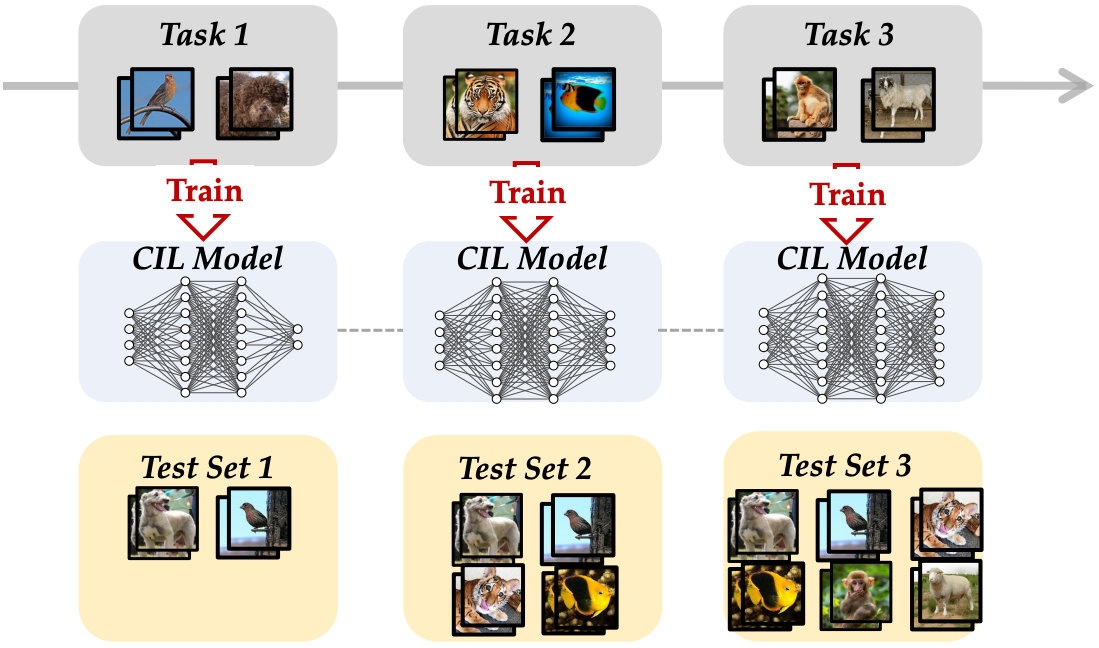
\includegraphics[width=0.9\columnwidth]{images/cil-setup.png}
    \end{center}
    \caption{General CIL setup \cite{zhou2021pycil}.}
    \label{fig:cil-setup}
\end{figure}

During the class incremental learning, a stream of class groups $\{\mathcal{Y}_t\}$ and their corresponding training data $\{\mathcal{D}_t\}$ are observed by the model. At step $t$, the incoming dataset $\{\mathcal{D}_t\}$ is of the form $(\textbf{x}_{\textbf{i}}^{\textbf{i}}, y_i^t)$ where $\textbf{x}_{\textbf{i}}^{\textbf{i}}$ is the input image and $y_i^t \in \mathcal{Y}_t$ is the label set $\mathcal{Y}_t$. The label space of the model consists in all the seen categories $\tilde{\mathcal{Y}}_t = \cup_{i=1}^t \mathcal{Y}_i$ and a good model should predict well on all classes $\tilde{\mathcal{Y}}_t$. As described in \autoref{sec:cil-methods}, some CIL algorithms save a part of data at timestamp $t$ as the memory $\mathcal{M}_t$ for future training. The CIL setup is shown in \autoref{fig:cil-setup}

\subsection{Methods}
\label{sec:cil-methods}


\begin{figure}
    \centerline{
        \begin{forest} for tree={align=center, inner sep=2pt}
        [Class Incremental Learning (CIL)\\methods
        [Replay\\methods
            [Rehearsal
            [
                iCaRL \cite{rebuffi2017icarl}\\
                ER \cite{rolnick2019experience}\\
                SER \cite{isele2018selective}\\
                TEM \cite{chaudhry2019continual}\\
                CoPE \cite{de2021continual}
            ]
            ]
            [Pseudo\\Rehearsal
            [
                DGR \cite{shin2017continual}\\
                PR \cite{atkinson1802pseudo}\\
                CCLUGM \cite{lavda2018continual}\\
                LGM \cite{ramapuram2020lifelong}\\
            ]
            ] 
            [Constrained
            [
                GEM \cite{lopez2017gradient}\\
                A-GEM \cite{chaudhry2018efficient}\\
                GSS \cite{aljundi2019online}\\
            ]
            ] 
        ]
        [Regularization-based\\methods
        [Prior-focused 
            [
                EWC \cite{kirkpatrick2017overcoming}\\
                IMM \cite{lee2017overcoming}\\
                SI \cite{zenke2017continual}\\
                R-EWC \cite{liu2018rotate}\\
                MAS \cite{aljundi2018memory}\\
                Riemannian Walk \cite{chaudhry2018riemannian}\\
            ]
        ]
        [Data-focused 
            [
            LwF \cite{li2017learning}\\
            LFL \cite{jung2016less}\\
            EBLL \cite{rannen2017encoder}\\
            DMC \cite{zhang2020class}\\
            ]
        ]
        ]
        [Parameter\\isolation methods
        [Fixed\\Network
            [
                PackNet \cite{mallya2018packnet}\\
                PathNet \cite{fernando2017pathnet}\\
                Piggybak \cite{mallya2018piggyback}\\
                HAT \cite{serra2018overcoming}\\
            ]
        ]
        [Dynamic\\Network
            [
                PNN \cite{rusu2016progressive}\\
                Expert Gate \cite{aljundi2017expert}\\
                RCL \cite{xu2018reinforced}\\
                DAN \cite{rosenfeld2018incremental}\\
            ]    
        ]]
        ]
        \end{forest}
    }
    \caption{CIL algorithms taxonomy presented in \cite{delange2021continual}.}
    \label{fig:cil-taxonomy}

\end{figure}


     

The problem of CIL has been addressed using different methods, but these methods can be divided into three main categories and their sub-categories. The taxonomy and the list of algorithms, summarized in the \autoref{fig:cil-taxonomy}, is based on these publications \cite{liu2021adaptive, delange2021continual}:

 

\begin{enumerate}
    \item \textbf{Replay methods}: These works stores samples of old classes which are replayed while learning a new task, by doing so it is possible to alleviate forgetting.
    The samples are either reused as model inputs for rehearsal, or to constrain optimization of the new task loss to prevent previous task interference.

    \begin{enumerate}
        \item \textit{Rehearsal} \cite{rebuffi2017icarl, rolnick2019experience, isele2018selective, chaudhry2019continual, de2021continual}: The model is retrained on a limited subset of stored samples.
        \item \textit{Pseudo Rehearsal} \cite{shin2017continual, atkinson1802pseudo, lavda2018continual, ramapuram2020lifelong}: Approximate previous tasks samples using either random input vector or more advanced techniques like generative models with the drawback of adding complexity to the system pipeline.
        \item \textit{Constrained optimization} \cite{lopez2017gradient, chaudhry2018efficient, aljundi2019online}: Update model's weights for the new task in such a way to not interfere with previous task weights.
    \end{enumerate}
    
    \item \textbf{Regularization-based methods}: These works do not store raw data and reduce the memory requirements. An extra regularization term is introduced in the loss function, in this way it is possible to learn new classes while maintaining the previous knowledge.
    \begin{enumerate}
        \item \textit{Prior-focused methods} \cite{kirkpatrick2017overcoming, lee2017overcoming, zenke2017continual, liu2018rotate, aljundi2018memory, chaudhry2018riemannian}: This approach tries to estimate the importance of the neural network parameters to avoid forgetting as much as possible. Then, when training on new tasks, the optimization process penalizes changes to important weights.
        \item \textit{Data-focused methods} \cite{li2017learning, jung2016less, zhang2020class, rannen2017encoder}: This approach uses knowledge distillation \cite{hinton2015distilling} treating the old model trained on the previous task as the teacher, and use it combined with the new data to train the student model.
    \end{enumerate}
    \item \textbf{Parameter isolation methods}: This class of methods use different model parameters for each task.
    \begin{enumerate}
        \item \textit{Fixed Network} \cite{mallya2018packnet, mallya2018piggyback, serra2018overcoming, fernando2017pathnet}: The model architecture is kept fixed and the knowledge is updated involving masks for the parameters' weights.
        \item \textit{Dynamic Architectures} \cite{rusu2016progressive, xu2018reinforced, aljundi2017expert, rosenfeld2018incremental}: The model architecture dynamically change after each incremental task, and the old parameters are freezed to prevent forgetting. Another approach is to dedicate a model to each incremental task
    \end{enumerate}
\end{enumerate}

Since there are several different algorithms for CIL, the work presented by Zhou et al. in \cite{zhou2021pycil} aims to compare a subset of these algorithms considering the same experimental setup. To this purpose, they publish a repository\footnote{PyCIL GitHub repository: \href{https://github.com/G-U-N/PyCIL}{https://github.com/G-U-N/PyCIL}}
on GitHub where they introduce \textit{PyCIL: A Python Toolbox for Class-Incremental Learning}, which is an implementation of all the following algorithms:

\begin{itemize}
    \item \textbf{Finetune}: The baseline method which simply updates parameters on new tasks and
    suffers from severe catastrophic forgetting.
    \item \textbf{Replay}: The baseline method which updates parameters on new task with instances
    from the new dataset and exemplar set.
    \item \textbf{EWC} \cite{kirkpatrick2017overcoming}: Uses Fisher Information Matrix to weigh the
    importance of each parameter and regularizes important parameters to overcome forgetting.
    \item \textbf{LwF} \cite{li2017learning}: Uses knowledge distillation (Hinton et al., 2015) to
    align the output probability between old and new model.
    \item \textbf{iCaRL} \cite{rebuffi2017icarl}: Uses knowledge distillation (Hinton et al., 2015) to
    align the output probability between old and new model. Besides, it also introduces
    exemplar set for rehearsal and uses nearest center mean classifier.
    \item \textbf{GEM} \cite{lopez2017gradient}: Uses exemplars as the regularization of
    gradient updating.
    \item \textbf{BiC} \cite{wu2019large}: Trains an extra adaptation layer based on iCaRL, which
    adjusts the logits on new classes.
    \item \textbf{WA} \cite{zhao2020maintaining}: Normalizes the classifier weight after each learning session
    based on iCaRL.
    \item \textbf{PODNet} \cite{douillard2020podnet}: Introduces a novel distillation loss (Pooled
    Outputs Distillation) constraining the whole convolutional network.
    \item \textbf{DER} \cite{yan2021dynamically}: A two-stage learning approach that utilizes a dynamically
    expandable representation for more effective incremental concept modeling.
    \item \textbf{Coil} \cite{zhou2021co}: Builds bi-directional knowledge transfer in the classincremental learning process with optimal transport (Villani, 2008). It first addresses
    the ability that old model can help learning new classes.
\end{itemize}

The CIL algorithms are tested on two different benchmark datasets, i.e. CIFAR100 and ImageNet100. These datasets are composed of 100 classes and the experiments performed by \cite{zhou2021pycil} adopt this CIL setup: 10 classes for the initial stage followed by 9 incremental learning iterations consisting of 10 new classes. Then, the top-1 accuracy is reported for all the incremental stages.
The results are shown in \autoref{fig:cil-comaprison} and the top-1 accuracy at the final stage is reported in \autoref{table:cil-results}.


\begin{table}
    \centering
    \begin{tabular}{c c} 
     \hline
     \textbf{Method} & \textbf{Top-1 accuracy} \\
     & \textbf{(last stage)}\\
     \hline
     Finetune & 26.25 \\ 
    Replay & 59.31 \\ 
    GEM & 40.18 \\ 
    LwF & 43.56 \\ 
    iCaRL & 64.42 \\ 
    EWC & 29.73 \\ 
    WA & 67.09 \\ 
    PODNet & 55.22 \\ 
    BiC & 65.08 \\ 
    Coil & 65.48 \\ 
    DER & 69.74 \\ 

     \hline
    \end{tabular}
    \caption{Top-1 accuracy of the CIL algorithms at the $10$-th incremental stage using the CIFAR100 dataset. \cite{zhou2021pycil}.}
    \label{table:cil-results}
    \end{table}

From the results reported by \cite{zhou2021pycil} in \autoref{fig:cil-comaprison} it is clear that 


\subsection{DER: an algorithm for class incremental learning}
\subsubsection{Algorithm description}
\subsubsection{Weight aligning}
\subsubsection{Masking and pruning}
